\newprob{1716014275}
{
    一針筒載有單原子理想氣體。活塞與針筒內壁之 間的摩擦力頗大,不可忽略。
    % \\A syringe contains some monatomic ideal gas. The friction between its inner walls and its piston is not negligible.
    \begin{figure}[h!]
        \centering
        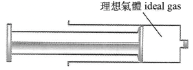
\includegraphics[width=.3\textwidth]{assets/a51301c5.png}
    \end{figure}
    \begin{parts}
        \part 把氣體由 \oc{0} 加熱至 \oc{50},活塞全程皆靜 止不動。試草繪一線圖,以顯示氣體總內能 的增幅如何隨温度 $\theta$ 轉變。
        % \\The gas is heated from \oc{0} to \oc{50} without the piston moving. Sketch a graph to show how the total internal energy gain of the gas changes with the temperature $\theta$. \zhtwo{2}
        % \begin{solutionorbox}
        %     [\stretch{3}]

        % \end{solutionorbox}
        \part 繼續加熱氣體,活塞便漸漸移動。氣體最後 加熱至\oc{100}。在同一線圖上,以虛線表示氣體內能在 $\theta$ =\oc{50}至 $\theta$ =\oc{100} 之間的變化。假設活塞所受的摩擦力不變。
        % \\The gas is further heated and the piston starts to move. The final temperature is \oc{100}. Sketch on the same graph, using dotted line, to show how the internal energy gain changes with the temperature $\theta$ from \oc{50} to \oc{100}. Assume that the friction is constant when the piston moves. \zhtwo{1}
        % \begin{solution}
        %     [\stretch{2}]
        % \end{solution}
    \end{parts}
}{
    \sol\par
    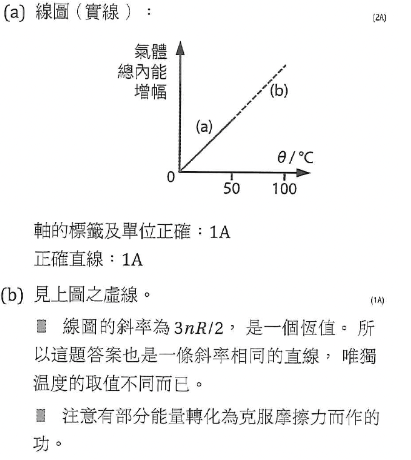
\includegraphics[width=.6\textwidth]{assets/830ce5dd.png}
}
\newprob{1716013866}
{
    有四種貴族氣體:氦、氖、氬和氪。這些氣體是單原子的,並被假設為理想氣體。這四種原子的質量比約為1:5:10:21。
    % \\There are four noble gases: helium, neon, argon and Krypton. The gases are monatomic and are assumed to behave as ideal gases. The mass ratio of the four types of atoms is about 1:5:10:21.
    \begin{parts}
        \part 假定氣體的溫度相同,證明氣體原子速度平方值的平均與每個原子的質量成反比。\zzh{3}
        % \\Assume the temperatures of the gases are the same. Show that the mean of the square values of the speeds of the gas atoms is inversely proportional to the mass of each atom.
        % \begin{solutionordottedlines}
        %     [\stretch{3}]

        % \end{solutionordottedlines}
        \part 哪種氣體的原子具有最低的方均根速率?
        % \\Which gas has atoms with the lowest root mean square speed? 
        \zzh{1}
        % \begin{solutionordottedlines}
        %     [\stretch{1}]
        %     \begin{itemize}
        %         \item 
        %     \end{itemize}
        % \end{solutionordottedlines}
        \part 在某一溫度下,氖原子的方均根速率為 \qty{609}{m.s^{-1}}。求此溫度下氪原子的方均根速率。
        % \\The root mean square speed of neon atoms at a certain temperature is \qty{609}{m.s^{-1}}. Find the root mean square speed of krypton atoms at this temperature. 
        \zzh{3}
        % \begin{solutionordottedlines}
        %     [\stretch{3}]

        % \end{solutionordottedlines}
    \end{parts}
}{
    \sol\begin{enumerate}[label=(\alph*)]
        \item \topalign{\par
                  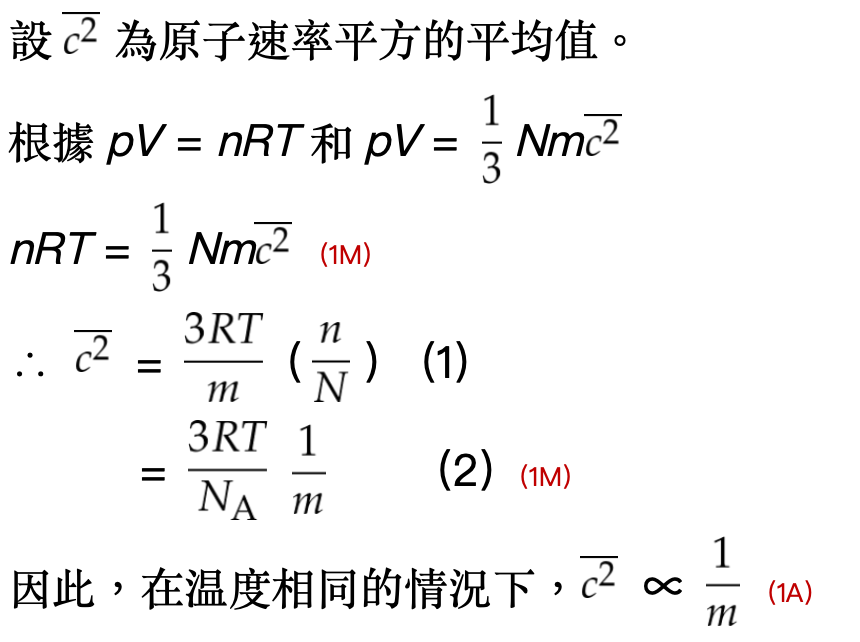
\includegraphics[width=.5\textwidth]{assets/8677e05b.png}
                  \par}
        \item  氪氣 \giveA
        \item  \topalign{\par
                  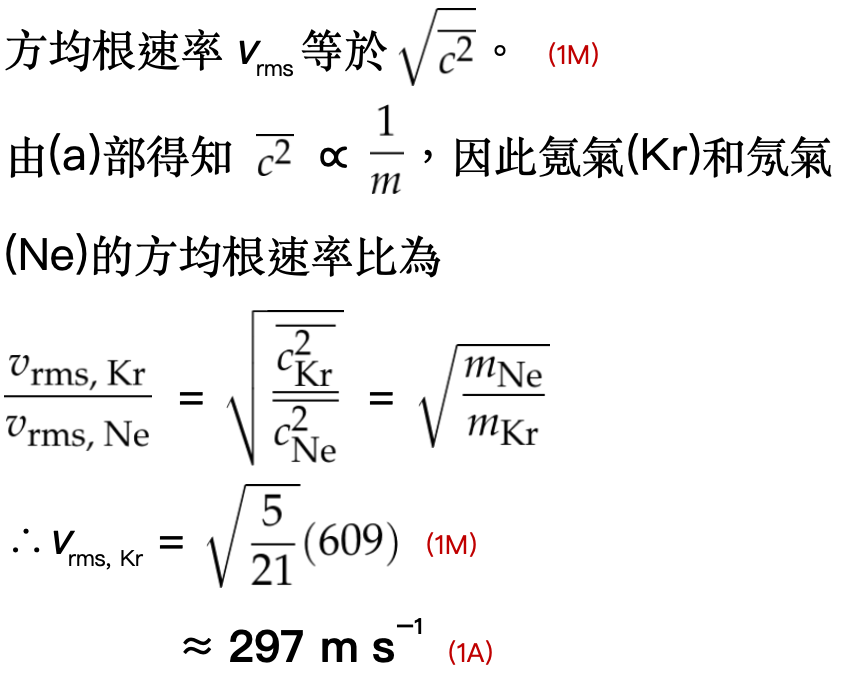
\includegraphics[width=.5\textwidth]{assets/d9e8816b.png}
                  \par}
    \end{enumerate}
}

\newprob{1716014162}
{
    一個高度為 2 m,橫截面積為 \qty{0.5}{m^2} 的圓柱形容器兩端被封閉。它被一個質量為250 kg 的無摩擦活塞分為兩個隔間。下部隔間內含有 0.2 mol 的理想氣體,而上部隔間則被抽真空。
    % \\A cylindrical container of height 2 m and cross-sectional area  \qty{0.5}{m^2}  is sealed at both ends. It is divided into two compartments by a frictionless piston of mass 250 kg. The lower compartment contains 0.2 mole of an ideal gas while the upper compartment is evacuated.
    \begin{figure}[h!]
        \centering
        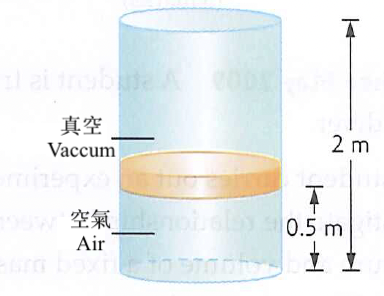
\includegraphics[width=.3\textwidth]{assets/f29c455c.png}
    \end{figure}
    \begin{parts}
        \part 初始時,活塞位於容器底部上方 0.5 m 處。求氣體的溫度T$_1$。
        % \\Initially, the piston is at 0.5 m above the bottom of the container. Find the temperature T$_1$ of the gas. 
        \zzh{3}
        % \begin{solutionordottedlines}
        %     [\stretch{3}]
        % \end{solutionordottedlines}
        \part 現在,氣體被一個內部加熱線圈(未顯示)慢慢加熱。最終氣體的溫度升高到 T$_2$,活塞上升到距容器底部 0.9 m 的位置。求
        % \\The gas is now slowly heated by an internal heating coil (not shown). Finally the gas temperature increases to T$_2$ and the piston moves up to 0.9 m above the bottom. Find
        \begin{subparts}
            \subpart T$_2$
            \subpart 氣體獲得的能量E。
            % \\the energy gained E by the gas.
        \end{subparts}
        \zzh{4}
        % \begin{solutionordottedlines}
        %     [\stretch{4}]
        % \end{solutionordottedlines}
        \part 現在氣體獲得了額外的能量800 J。問保持活塞在(b)處的高度不變所需的額外力量是多少?
        % \\Now the gas gains an additional energy of 800 J . What is the additional force required to keep the piston fixed at the height in (b)?
        \zzh{3}
        % \begin{solutionordottedlines}
        %     [\stretch{3}]
        % \end{solutionordottedlines}
    \end{parts}
    % \clearpage\begin{solutionordottedlines}
    %     [\stretch{3}]
    %     {\par
    %         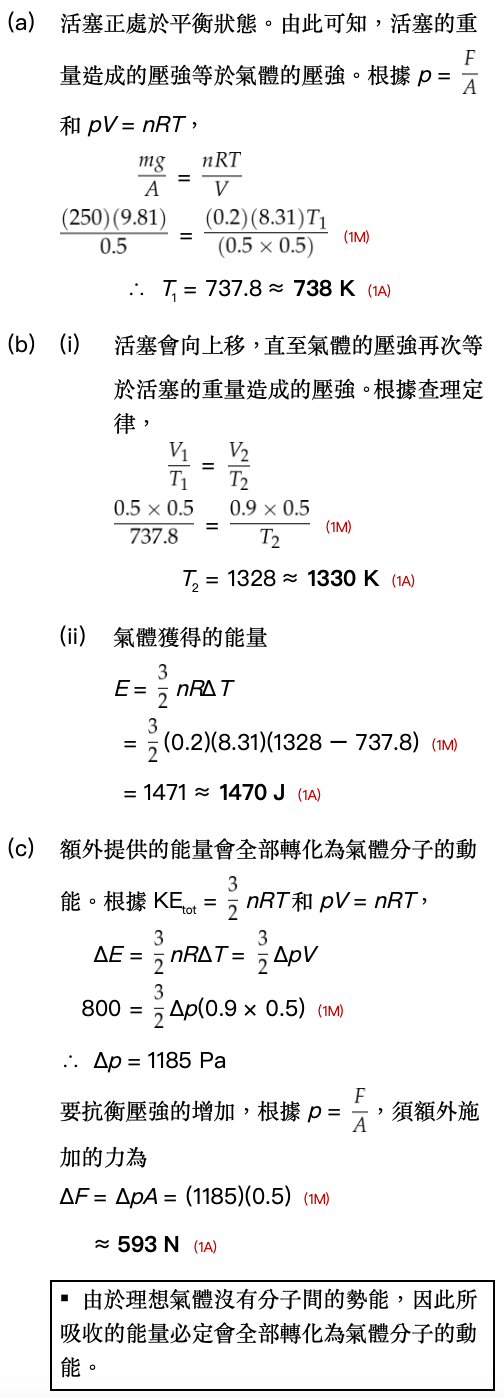
\includegraphics[width=.5\textwidth]{assets/79746d85.png}
    %         \par}
    % \end{solutionordottedlines}
}{
    \sol{\par
        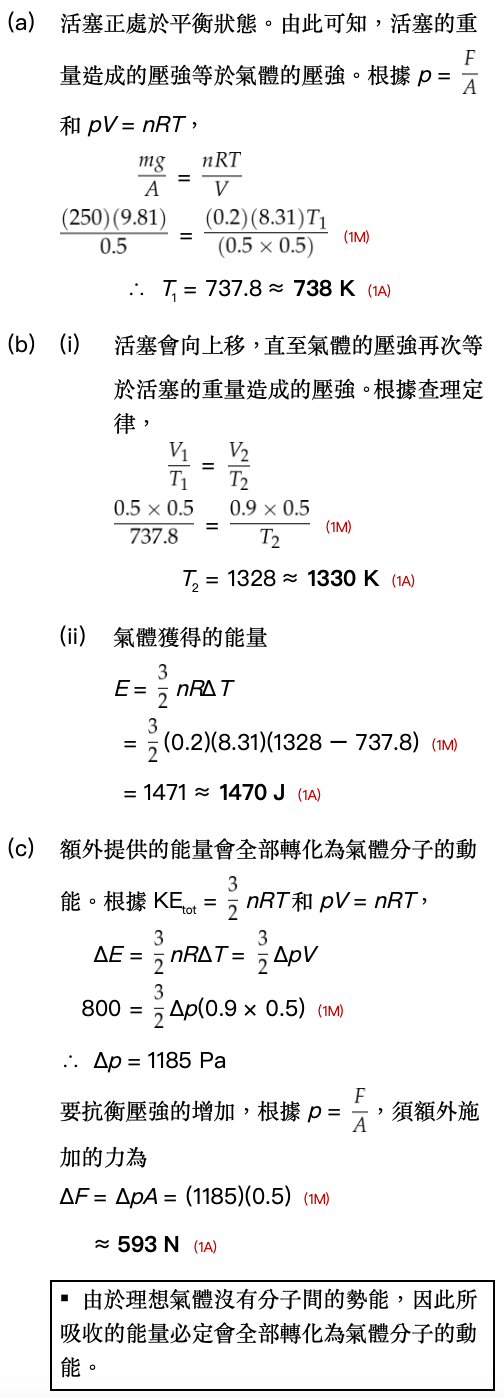
\includegraphics[width=.45\textwidth]{assets/79746d85.png}
        \par}
}

